\documentclass[11pt]{article}
\usepackage{tikz}
\usepackage{pgfplots}
\pgfplotsset{compat=1.18}
\usepackage[hidelinks]{hyperref}
\usepackage[a4paper,margin=25mm]{geometry}

\begin{document}
\title{Golden Baseline: TikZ and PGFPlots}
\author{Company Agent LaTeX Toolchain Lab}
\date{2026-10-26}
\maketitle

\section{Diagram}
The topology skeleton in Figure~\ref{fig:topology} and the decay curve in
Figure~\ref{fig:decay} render with PGFPlots. The compile must not require
shell escape, network access or external image files.

\begin{figure}[ht]
  \centering
  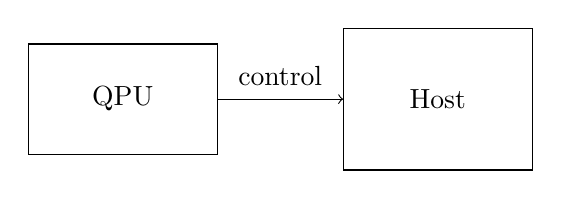
\begin{tikzpicture}
    \draw (0,0) rectangle (2.4,1.4);
    \node at (1.2,0.7) {QPU};
    \draw[->] (2.4,0.7) -- (4.0,0.7);
    \node at (3.2,1.0) {control};
    \draw (4.0,-0.2) rectangle (6.4,1.6);
    \node at (5.2,0.7) {Host};
  \end{tikzpicture}
  \caption{Control topology skeleton}
  \label{fig:topology}
\end{figure}

\begin{figure}[ht]
  \centering
  \begin{tikzpicture}
    \begin{axis}[
        width=9cm, height=6cm,
        xlabel={time (ns)}, ylabel={amplitude},
        domain=0:10, samples=41,
        xmin=0, xmax=10, ymin=0, ymax=1.1,
    ]
      \addplot[thick] {exp(-0.25*x)};
    \end{axis}
  \end{tikzpicture}
  \caption{Exponential decay curve}
  \label{fig:decay}
\end{figure}

\end{document}
